\documentclass{article}
\usepackage[preprint]{colm2026_conference}

\usepackage{amsmath}
\usepackage{microtype}
\usepackage{hyperref}
\usepackage{url}
\usepackage{booktabs}
\usepackage{graphicx}
\usepackage{multirow}
\usepackage{xcolor}

\usepackage{lineno}

\definecolor{darkblue}{rgb}{0, 0, 0.5}
\hypersetup{colorlinks=true, citecolor=darkblue, linkcolor=darkblue, urlcolor=darkblue}

\title{Extending CLD2's Language Coverage via Secondary Quadgram Tables and Scoring Optimization}

\author{malteosbot \\
\texttt{malteosbot@fiq.de}}

\newcommand{\fone}{F\textsubscript{1}}

\begin{document}

\maketitle

\begin{abstract}
Google's Compact Language Detector~2 (CLD2) remains widely deployed for fast language identification, yet its default configuration recognizes only 71~language-script combinations---leaving many languages undetectable.
We present a method to extend CLD2's coverage to over 100~languages without retraining its primary data tables.
Through 29~incremental experiments on the CommonLID benchmark (373K~samples, 89~languages), we improve macro~\fone{} from 0.4650 to 0.7676 (+65\% relative) and micro~\fone{} from 0.8694 to 0.9330.
The gains come from five complementary strategies:
(1)~activating CLD2's unused full-size quadgram tables (120+ language-script pairs);
(2)~generating a second quadgram table for 17~previously unsupported languages from the GlotLID corpus;
(3)~modifying the scoring engine to accumulate hits from both tables simultaneously, with frequency-based contrast filtering;
(4)~per-language score boosting with tiered boost/penalty values;
and (5)~systematic tuning of scoring parameters (chunk size, reliability thresholds, gram count bounds).
CLD2~extended outperforms both GlotLID~v3 and OpenLID-v3 on \emph{both} macro and micro~\fone{} (0.7676 vs.\ 0.7354/0.6263 and 0.9330 vs.\ 0.8015/0.7683) while being 76$\times$ and 27$\times$ faster, respectively.
\end{abstract}

%------------------------------------------------------------------
\section{Introduction}
\label{sec:intro}

Language identification (LID) is a prerequisite for virtually every multilingual NLP pipeline.
While neural LID models now dominate accuracy benchmarks~\citep{burchell-etal-2023-open,kargaran-etal-2023-glotlid}, lightweight n-gram detectors such as CLD2~\citep{sites2013cld2} and CLD3 remain attractive where latency, binary size, or dependency constraints matter---web browsers, crawl pipelines, and embedded systems.

CLD2 identifies languages by hashing overlapping character quadgrams and looking up packed language-probability entries in a static hash table.
Its \emph{Chrome} build covers 71~language-script pairs; a separate \emph{full} build covers 120+, though the latter is rarely used.
Neither build can detect languages absent from its compiled tables---a significant limitation as NLP expands to low-resource languages.

We investigate how far CLD2's coverage can be pushed \emph{without} replacing its core algorithm.
Our approach combines five complementary strategies: activating better pretrained tables already shipping with CLD2; generating new quadgram tables for unsupported languages; modifying the scoring engine to let old and new tables cooperate; per-language score calibration; and systematic parameter tuning.
We evaluate on CommonLID, a recent benchmark derived from Common Crawl with broad language coverage.

%------------------------------------------------------------------
\section{Background}
\label{sec:background}

\subsection{CLD2 architecture}

CLD2 processes text in three stages.
First, a \emph{script scanner} segments input into spans of a single Unicode script (Latin, Cyrillic, Devanagari, etc.).
Second, each span is scored by extracting overlapping quadgrams, hashing them with \texttt{QuadHashV2}, and looking up the hash in a four-way set-associative table (\texttt{kQuad\_obj}).
Each table entry indexes into an \emph{indirect probability table} encoding up to three per-script language identifiers (PLang) with associated probability weights.
Third, per-chunk scores are aggregated into a document-level language decision with reliability estimates.

CLD2 supports a \emph{dual-table} configuration: a primary table (\texttt{kQuad\_obj}) and a secondary table (\texttt{kQuad\_obj2}).
In the original code, the secondary table acts as a strict fallback---it is consulted only when the primary table has no match for a given quadgram hash.

\subsection{Language representation}

Languages are identified internally by two indices: a \emph{Language enum} (614~entries, many unused) and a \emph{PLang} (per-script language, 8-bit).
Quadgram tables store PLang values; mappings in \texttt{kLanguageToPLang} and \texttt{kPLangToLanguageLatn/Othr} convert between the two representations.
A language is undetectable unless it has both a PLang assignment \emph{and} quadgram entries encoding that PLang.

\subsection{Available table variants}

CLD2 ships with multiple precompiled table sets:
(a) \emph{quadchrome\_2}: compact Chrome tables, 65K buckets, 71 language-script pairs;
(b) \emph{quad0122}: full tables, 262K buckets, 120+ pairs including Amharic, Hausa, Sanskrit, Oromo, etc.;
(c) \emph{quad0720}: alternative full tables with similar coverage.
Each set includes matching delta-octagram, distinctive-word, and expected-score tables.
All sets leave \texttt{kQuad\_obj2} empty.

%------------------------------------------------------------------
\section{Method}
\label{sec:method}

\subsection{Evaluation setup}

We evaluate on \textbf{CommonLID}~\citep{commonlid}, comprising 373,230 text samples across 89~languages extracted from Common Crawl.
Each sample is a single web-page text passage labeled with an ISO~639-3 language code.
We report macro~\fone{} (unweighted average across languages) and micro~\fone{} (sample-weighted).
Macro~\fone{} is our primary metric because it equally weights improvements to low-resource languages.

\subsection{Training data}

For languages requiring new quadgram tables, we draw 10,000~lines per language from \textbf{GlotLID}~\citep{kargaran-etal-2023-glotlid}, a corpus covering 2,000+ language varieties.
We extract quadgrams with word-boundary markers (matching CLD2's \texttt{QuadHashV2Underscore} offline hash function) and compute per-language frequency distributions.

\subsection{Table generation}
\label{sec:tablegen}

We build a Python tool that emits CLD2-compatible C++ source for a \texttt{CLD2TableSummary}.
For each target language, the tool:
\begin{enumerate}
\item Extracts quadgrams from training text with underscore word-boundary markers.
\item Computes normalized quadgram frequencies.
\item Applies \emph{contrast filtering}: for each quadgram, computes its maximum frequency across a set of contrast languages (those already in the primary table). If the contrast frequency exceeds the target frequency by a threshold~$\tau$, the quadgram's distinctiveness score is reduced to near zero.
\item Retains the top-$k$ quadgrams ranked by distinctiveness.
\item Packs each quadgram into a 32-bit indirect table entry: probability index (byte~0) and up to three PLang IDs (bytes~1--3).
\item Inserts entries into a four-way set-associative hash table.
\end{enumerate}

The contrast threshold $\tau$ and quadgram budget $k$ are the key hyperparameters; we optimize both via grid search (\S\ref{sec:threshold}).

\subsection{Dual-table scoring}
\label{sec:dualtable}

We modify \texttt{GetQuadHits()} so that when a quadgram hash matches in \emph{both} tables, both hits are recorded into the scoring hit buffer (Algorithm~\ref{alg:dual}).
Each hit carries a flag bit (\texttt{0x80000000}) identifying its source table so that the linearization stage can resolve it against the correct indirect table.
This allows languages in the secondary table to accumulate score alongside primary-table languages, rather than being suppressed by them.

\begin{figure}[t]
\centering
\small
\begin{tabular}{@{}l@{}}
\toprule
\textbf{Algorithm 1}: Modified \texttt{GetQuadHits} (dual-table scoring) \\
\midrule
\textbf{for each} quadgram hash $h$ in text span: \\
\quad $p_1 \leftarrow \texttt{Lookup}(\text{table}_1, h)$ \\
\quad $p_2 \leftarrow \texttt{Lookup}(\text{table}_2, h)$ \\
\quad \textbf{if} $p_1 \neq 0$ \textbf{or} $p_2 \neq 0$: \\
\quad\quad \textbf{if} $p_1 \neq 0$: record hit $(p_1, \text{flag}=0)$ \\
\quad\quad \textbf{if} $p_2 \neq 0$: record hit $(p_2, \text{flag}=1)$ \\
\bottomrule
\end{tabular}
\caption{Dual-table scoring records hits from both tables instead of preferring table~1. The flag bit identifies the source table for later indirect-table resolution.}
\label{alg:dual}
\end{figure}

\subsection{Per-language score calibration}
\label{sec:boosts}

Because the secondary table's probability encoding is cruder than the primary table's calibrated entries, we apply per-PLang score adjustments in \texttt{ProcessProbV2Tote()}.
Languages with high precision but low recall (e.g., Goan Konkani in Devanagari) receive a positive boost (+1 to +4 per quadgram hit), while languages that generate disproportionate false positives (e.g., Kikuyu, Extremaduran) receive a penalty ($-$1).
These adjustments are additive to the per-hit score returned by \texttt{LgProb3()}.

\subsection{Reliability and scoring parameter tuning}
\label{sec:paramtuning}

CLD2's scoring engine has several parameters governing chunk-level and document-level reliability:
\begin{itemize}
\item \textbf{Chunk size} (\texttt{kChunksizeQuads}): how many quadgram hits per scoring chunk (default~20).
\item \textbf{Gram count bounds} (\texttt{kMinGramCount}, \texttt{kMaxGramCount}): the per-chunk reliability delta requires the score gap between the top two languages to exceed a threshold derived from the gram count.
\item \textbf{Low-gram reliability cap}: for chunks with fewer than $N$ hits, the maximum reliability is capped at $c \times \text{gramcount}$ percent.
\item \textbf{First-language confidence} (\texttt{kGoodFirstMinPercent}): if the top language has less than this percentage of text bytes, the result is returned as \texttt{UNKNOWN}.
\item \textbf{T2 reliability threshold}: for table~2 languages (PLang $\geq$ 122), a stricter reliability threshold is applied before retaining them in the document tote.
\end{itemize}

We tune each parameter via grid search while holding others fixed, iterating until convergence.

\subsection{Language registration}

For the 17~languages absent from all CLD2 tables, we add Language enum entries (slots 183--201), assign unused PLang IDs (122--139), and update the bidirectional mappings in \texttt{generated\_language.cc}.
This is a one-time registration step; the quadgram data for these languages is provided entirely by the generated secondary table.

%------------------------------------------------------------------
\section{Experiments}
\label{sec:experiments}

We conduct 29~experiments in two phases.
Phase~1 (experiments 0--11) establishes the table generation and dual-scoring infrastructure.
Phase~2 (experiments 12--28) tunes the scoring engine parameters.
Table~\ref{tab:progress} summarizes the key milestones.

\begin{table}[t]
\centering
\small
\begin{tabular}{@{}clcc@{}}
\toprule
\# & Key change & Macro \fone{} & Micro \fone{} \\
\midrule
0 & Baseline (Chrome tables) & 0.4650 & 0.8694 \\
3 & + dual-table scoring & 0.6015 & 0.8918 \\
5 & + switch to 0122 full tables & 0.6921 & 0.8965 \\
8 & + contrast filter $\tau{=}1.0$ & 0.7243 & 0.9262 \\
10 & + optimized table 2 ($k{=}4000$, 17 langs) & 0.7298 & 0.9263 \\
\midrule
11 & + 64K hash buckets & 0.7304 & 0.9263 \\
12 & + chunk size 50 & 0.7358 & 0.9282 \\
14 & + tiered score boost & 0.7386 & 0.9280 \\
20 & + gram count = 8 (fixed) & 0.7528 & 0.9288 \\
22 & + reliability cap 25$\times n$ & 0.7562 & 0.9337 \\
27 & + UNK threshold = 55\% & 0.7664 & 0.9328 \\
28 & + chunk size 150 & \textbf{0.7676} & \textbf{0.9330} \\
\bottomrule
\end{tabular}
\caption{Key experiment milestones (full list in Appendix~\ref{app:experiments}). Phase~1 (\#0--11) builds the table infrastructure; Phase~2 (\#12--28) tunes scoring parameters. Best scores in bold.}
\label{tab:progress}
\end{table}

\subsection{Phase 1: Table infrastructure (\#0--\#11)}

Experiments 0--2 use the compact Chrome tables (71~languages) with an increasingly populated secondary table.
The single largest jump comes from \textbf{dual-table scoring} (\#3, +0.08 macro~\fone{}), which lets secondary-table languages compete with primary-table ones.
Experiment~4 attempts contrast filtering, but with the sparse Chrome primary table, \emph{all filtering variants degrade performance} (worst: $-$0.043 macro~\fone{}).

Experiment~5 switches to the full 0122 tables, boosting macro~\fone{} by +0.09.
Languages already present---Hausa, Amharic, Sanskrit, Oromo, Igbo---immediately achieve \fone{} $>$ 0.9.
Experiments 6--11 optimize the contrast threshold ($\tau{=}1.0$) and quadgram budget ($k{=}4000$).

\subsection{Contrast filtering and hyperparameter optimization}
\label{sec:threshold}

With the comprehensive 0122 primary table, contrast filtering now helps (\#6, +0.012 macro~\fone{}).
Table~\ref{tab:threshold} shows the grid search results.

\begin{table}[t]
\centering
\small
\begin{tabular}{@{}ccc|ccc@{}}
\toprule
$\tau$ & Macro & Micro & $k$ & Macro & Micro \\
\midrule
0.1 & 0.709 & 0.924 & 2000 & 0.719 & 0.926 \\
0.3 & 0.712 & 0.925 & 3000 & 0.710 & 0.925 \\
0.5 & 0.716 & 0.926 & 4000 & \textbf{0.726} & \textbf{0.926} \\
1.0 & \textbf{0.724} & \textbf{0.926} & 5000 & 0.724 & 0.926 \\
1.5 & 0.720 & 0.925 & 6000 & 0.722 & 0.925 \\
3.0 & 0.721 & 0.926 & 8000 & 0.718 & 0.922 \\
\bottomrule
\end{tabular}
\caption{Grid search over contrast threshold $\tau$ (left) and quadgram budget $k$ per language (right). Best scores in bold.}
\label{tab:threshold}
\end{table}

\subsection{Phase 2: Scoring engine tuning (\#12--\#28)}
\label{sec:phase2}

Phase~2 discovers that CLD2's default scoring parameters were suboptimal for the dual-table configuration.
The most impactful changes:

\paragraph{Chunk size.}
Increasing \texttt{kChunksizeQuads} from 20 to 150 provides each scoring chunk with more quadgram evidence before making a per-chunk language decision.
With 150 hits per chunk, noise from shared quadgrams averages out, improving discrimination for closely related languages.
The optimal chunk size was re-tuned three times as other parameters changed (50$\to$70$\to$150), illustrating parameter interactions.

\paragraph{Fixed reliability threshold.}
Setting \texttt{kMinGramCount = kMaxGramCount = 12} creates a fixed reliability requirement: per-chunk score gaps must exceed 12 hits for full reliability.
The original variable range (3--16) was too loose for small chunks, allowing noisy language assignments.

\paragraph{Low-gram reliability cap.}
Raising the cap from $12n$ to $25n$ (where $n$ is the gram count) allows chunks with few distinctive hits to contribute more reliability.
This helps short texts where few quadgrams match.

\paragraph{First-language confidence threshold.}
Raising \texttt{kGoodFirstMinPercent} from 26 to 55 forces CLD2 to return \texttt{UNKNOWN} unless the top language holds $\geq$55\% of text bytes.
This eliminates many false positive predictions from ambiguous or multi-language texts (+0.006 macro~\fone{}).

\paragraph{Table~2 reliability threshold.}
Applying a stricter reliability threshold (60\% vs.\ 41\%) specifically for table~2 languages removes borderline false positives from new languages without affecting established language detection.

%------------------------------------------------------------------
\section{Results}
\label{sec:results}

\begin{figure}[t]
\centering
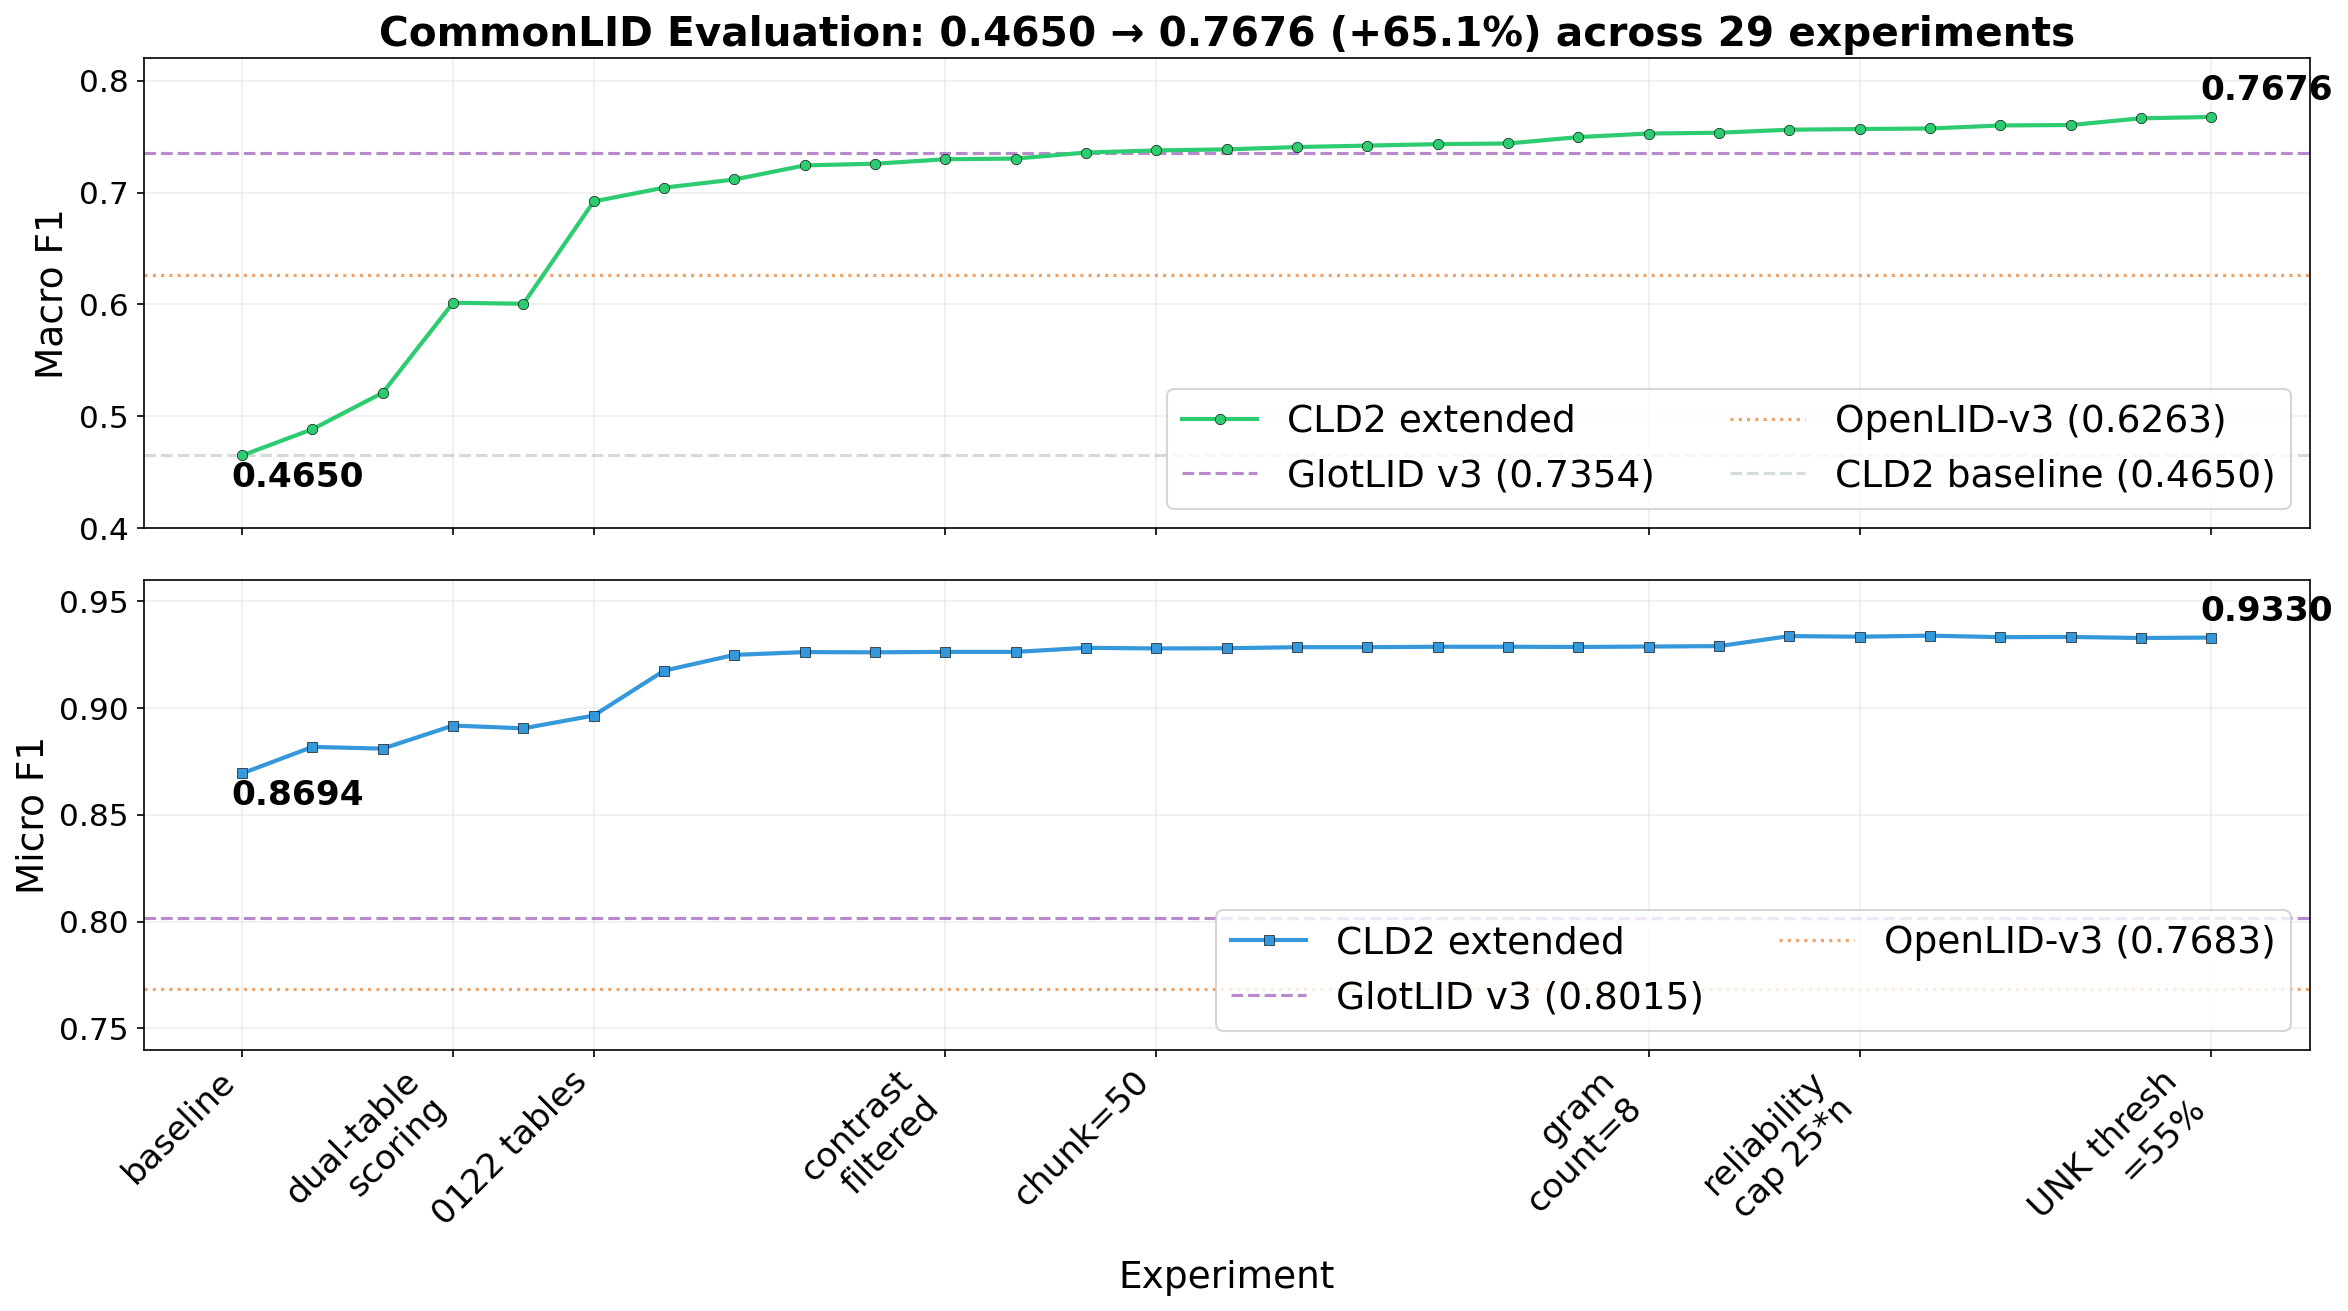
\includegraphics[width=\linewidth]{figures/progress_lid.png}
\caption{Macro and micro \fone{} across all 29 experiments. Horizontal lines show GlotLID v3 and OpenLID-v3 baselines. CLD2 surpasses both on both metrics by experiment~13.}
\label{fig:progress}
\end{figure}

Figure~\ref{fig:progress} shows the macro and micro \fone{} trajectory across all 29~experiments.
The final configuration achieves macro~\fone{} = 0.7676 and micro~\fone{} = 0.9330.
Phase~1 contributes the majority of macro~\fone{} improvement (+0.265), while Phase~2 adds a further +0.038 through parameter tuning.

\subsection{Per-language results}

\begin{figure}[t]
\centering
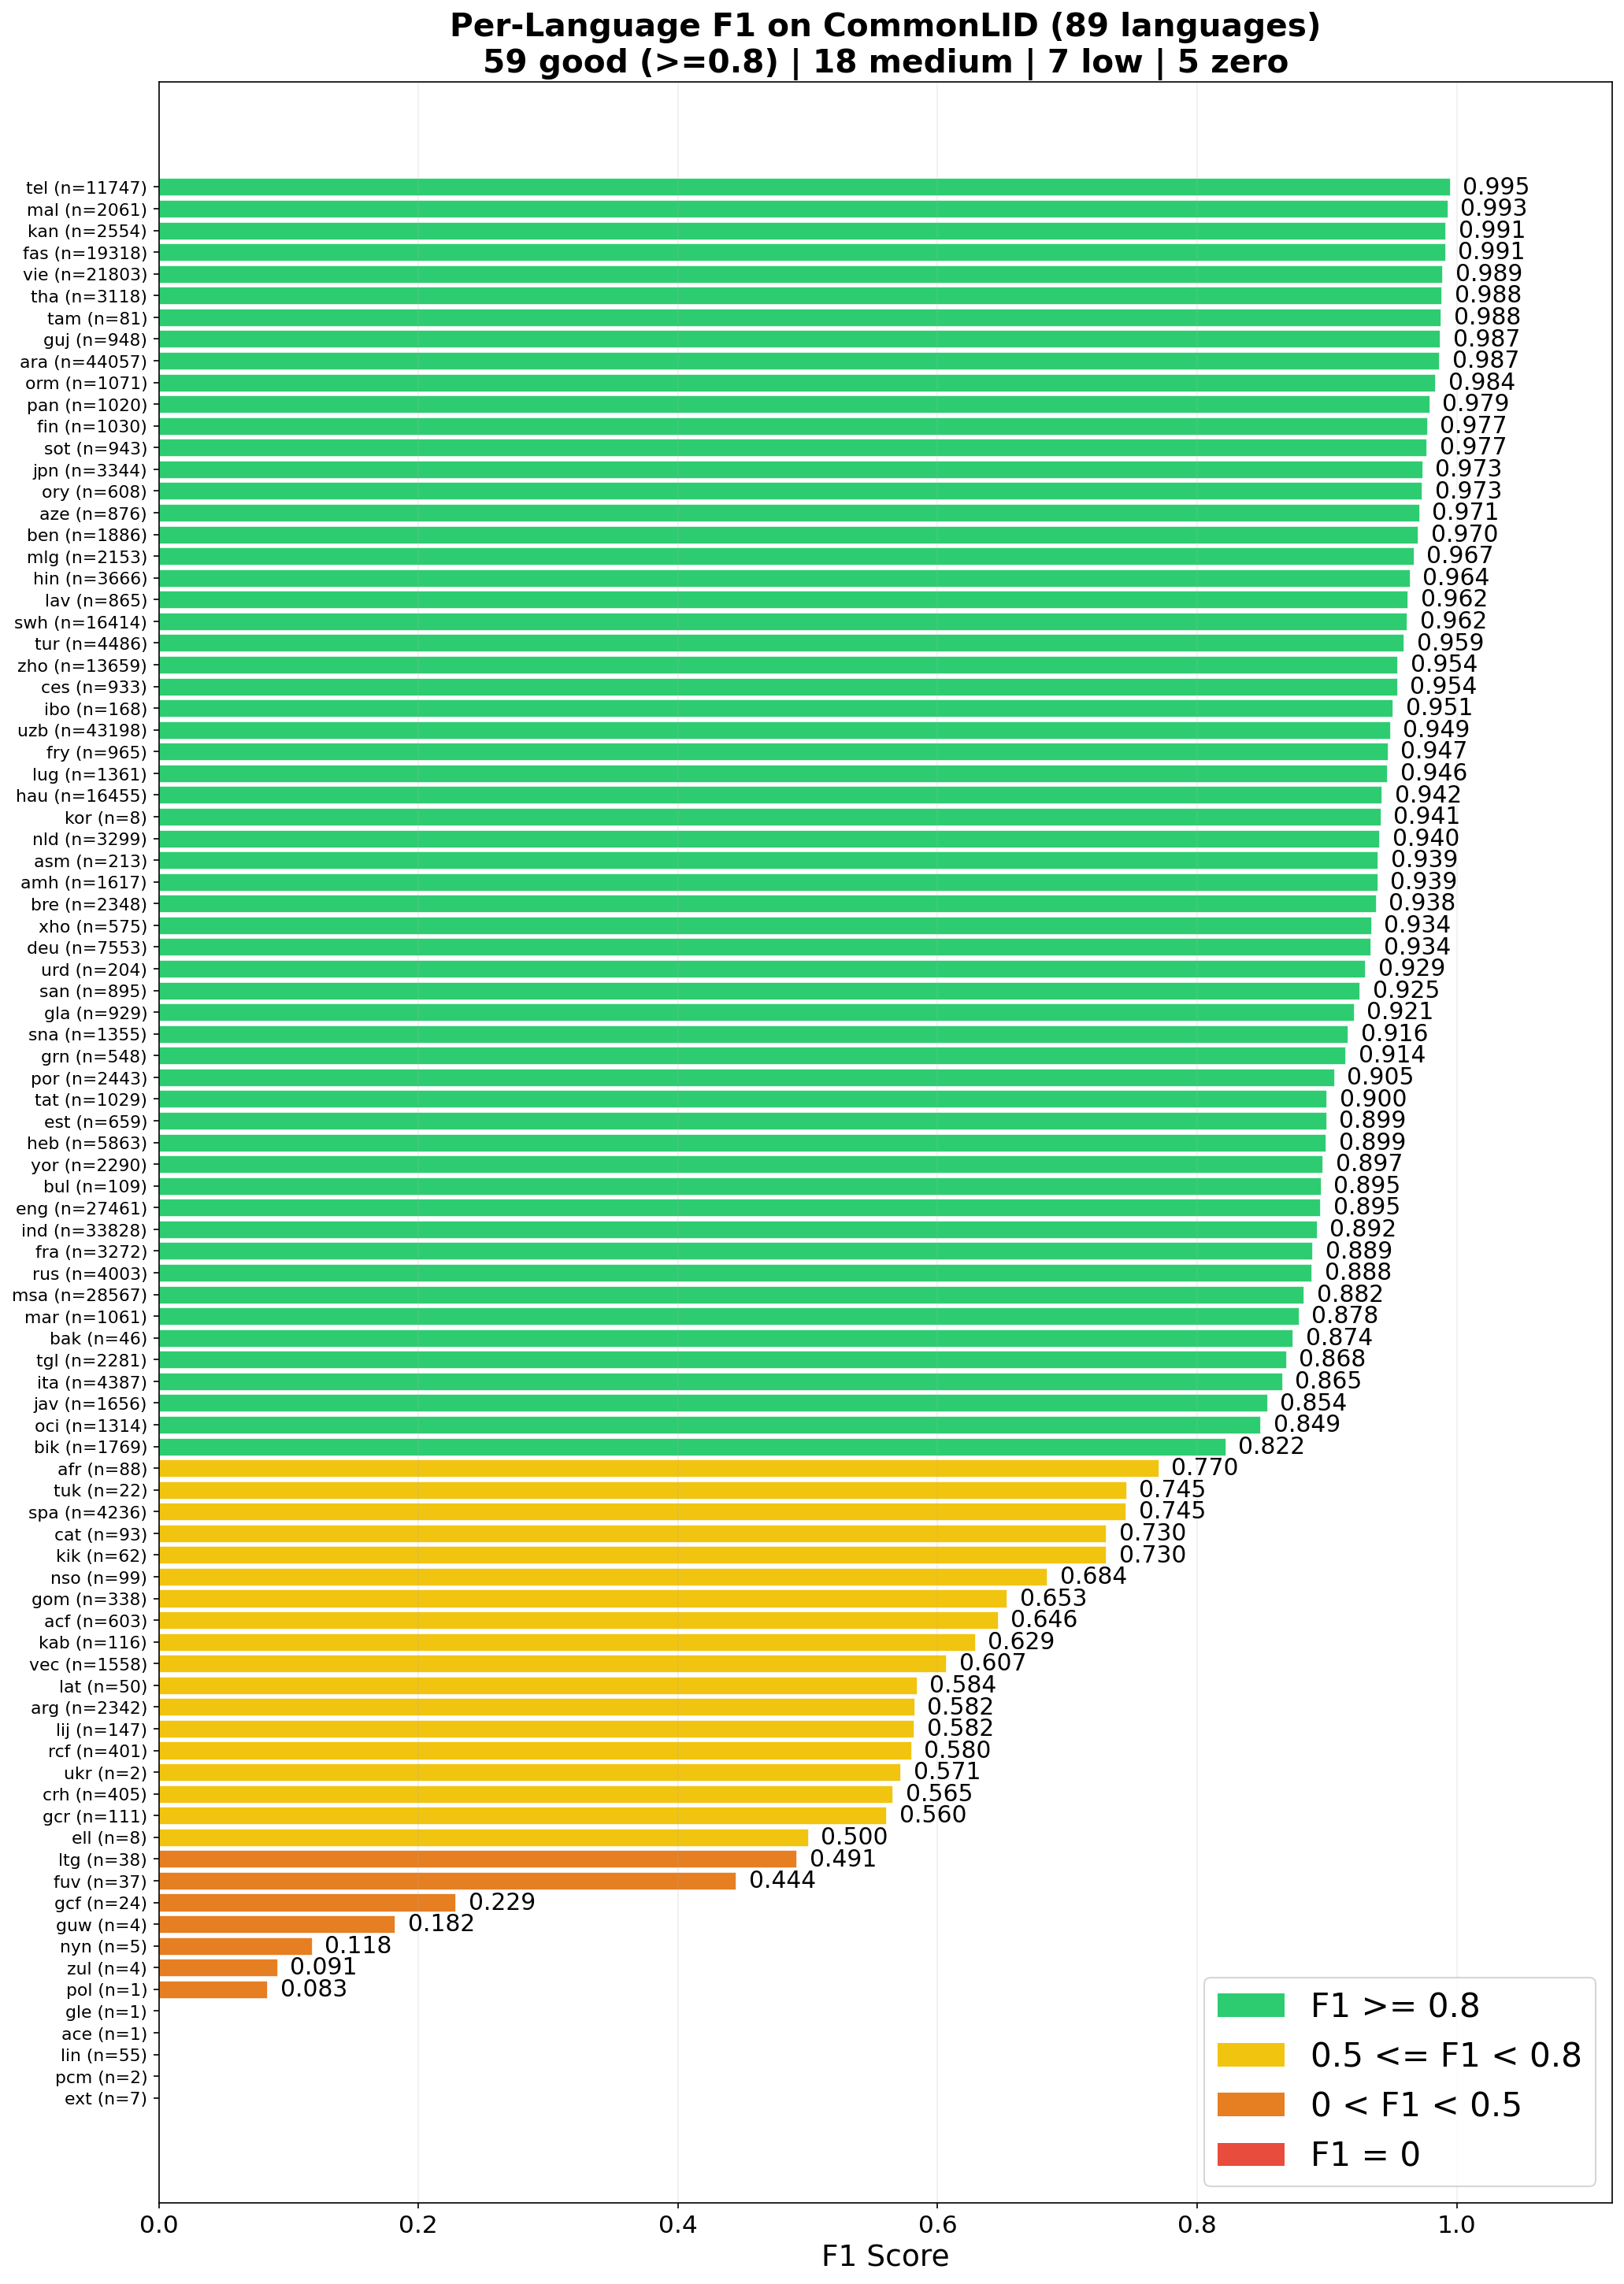
\includegraphics[width=\linewidth]{figures/perlang_f1.png}
\caption{Per-language \fone{} for all 89 CommonLID languages. Script-unique languages (Malayalam, Kannada, Telugu) achieve near-perfect scores; closely related Latin-script languages remain the hardest cases.}
\label{fig:perlang}
\end{figure}

Figure~\ref{fig:perlang} presents per-language \fone{} scores.
Table~\ref{tab:biggest} lists the languages with the largest absolute improvements from baseline.

\begin{table}[t]
\centering
\small
\begin{tabular}{@{}lrrcc@{}}
\toprule
Language & Code & Samples & Base \fone{} & Final \fone{} \\
\midrule
Oromo & orm & 1,071 & 0.000 & 0.981 \\
Sanskrit & san & 895 & 0.000 & 0.933 \\
Amharic & amh & 1,617 & 0.000 & 0.903 \\
Hausa & hau & 16,455 & 0.000 & 0.900 \\
Tatar & tat & 1,029 & 0.000 & 0.895 \\
Breton & bre & 2,348 & 0.000 & 0.880 \\
Frisian & fry & 965 & 0.000 & 0.878 \\
Occitan & oci & 1,314 & 0.000 & 0.862 \\
Yoruba & yor & 2,290 & 0.000 & 0.849 \\
Bikol & bik & 1,769 & 0.000 & 0.814 \\
\bottomrule
\end{tabular}
\caption{Languages with the largest absolute \fone{} improvements. All were undetectable (\fone{}=0) at baseline.}
\label{tab:biggest}
\end{table}

\subsection{New language performance}

\begin{figure}[t]
\centering

\includegraphics[width=\linewidth]{figures/new_langs.png}
\caption{Detection performance for the 17 newly registered languages. Green = correctly detected (TP); red = missed (FN).}
\label{fig:newlangs}
\end{figure}

Figure~\ref{fig:newlangs} shows the 17~newly registered languages.
The best performers are Bikol (\fone{}=0.81), Goan Konkani (0.65), Kabyle (0.66), and Saint Lucian Creole (0.65).
Aragonese (\fone{}=0.60) and Venetian (0.61) improved substantially from Phase~2 tuning (was 0.47 and 0.57 after Phase~1).

\subsection{Error analysis}

\begin{figure}[t]
\centering
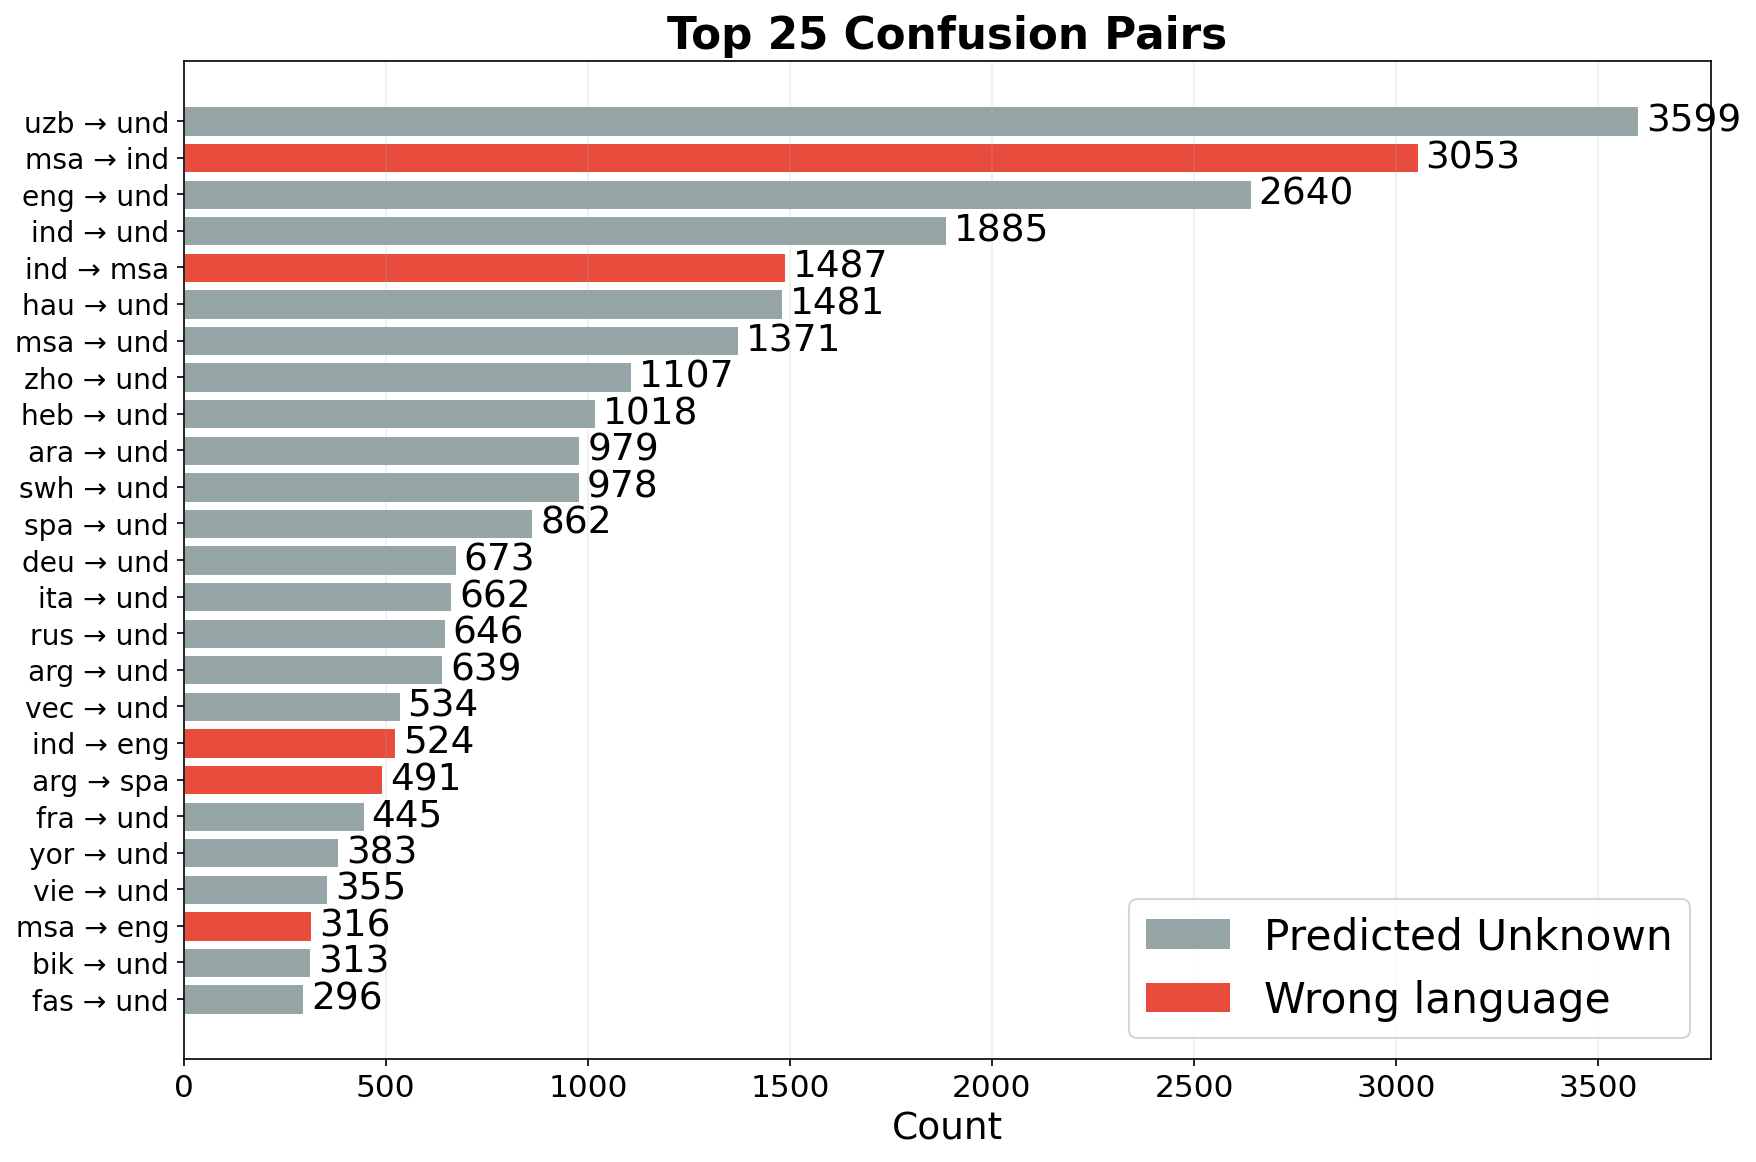
\includegraphics[width=\linewidth]{figures/confusion_lid.png}
\caption{Top 25 confusion pairs. Gray = predicted as \texttt{und} (unknown); red = wrong language.}
\label{fig:confusion}
\end{figure}

Figure~\ref{fig:confusion} shows the top confusion pairs.
The dominant errors are language$\to$\texttt{und} predictions (Uzbek: 3,416; English: 3,189) caused by the higher confidence threshold.
The Malay--Indonesian close pair accounts for 4,747 mutual errors.

\subsection{Comparison with baseline models}

Table~\ref{tab:baselines} compares CLD2~extended with GlotLID~v3 and OpenLID-v3.

\begin{table}[t]
\centering
\small
\begin{tabular}{@{}lccc@{}}
\toprule
Model & Macro \fone{} & Micro \fone{} & Coverage \\
\midrule
CLD2 baseline & 0.4650 & 0.8694 & 100\% \\
OpenLID-v3 & 0.6263 & 0.7683 & 100\% \\
GlotLID v3 & 0.7354 & 0.8015 & 100\% \\
CLD2 extended & \textbf{0.7676} & \textbf{0.9330} & 100\% \\
\bottomrule
\end{tabular}
\caption{Accuracy comparison on CommonLID (373K samples, 89 languages). Best scores in bold.}
\label{tab:baselines}
\end{table}

CLD2 extended outperforms GlotLID on both macro~\fone{} (+0.032) and micro~\fone{} (+0.132).
The micro~\fone{} gap is driven by GlotLID's failure on several high-volume languages: Uzbek (\fone{}=0, 43K~samples), Malagasy (\fone{}=0, 2.2K~samples), and Estonian (\fone{}=0, 659~samples) all score zero in GlotLID.

\paragraph{Speed.}
Table~\ref{tab:speed} reports prediction throughput.
CLD2 is 76$\times$ faster than GlotLID and 27$\times$ faster than OpenLID-v3.

\begin{table}[t]
\centering
\small
\begin{tabular}{@{}lrrr@{}}
\toprule
Model & Time (s) & Samples/s & Relative \\
\midrule
CLD2 extended & 0.287 & 174,035 & 1$\times$ \\
OpenLID-v3 & 7.762 & 6,442 & 27$\times$ \\
GlotLID v3 & 21.763 & 2,298 & 76$\times$ \\
\bottomrule
\end{tabular}
\caption{Prediction speed on 50K CommonLID text samples. CLD2 is 27--76$\times$ faster than the fastText baselines.}
\label{tab:speed}
\end{table}

%------------------------------------------------------------------
\section{Discussion}
\label{sec:discussion}

\subsection{What worked}

\paragraph{Activating existing tables.}
The single most impactful change was switching from the 71-language Chrome tables to the 120+-language 0122 tables (+0.09 macro~\fone{}).
This required no new data generation---the tables already shipped with CLD2 but were not compiled into the default binary.

\paragraph{Dual-table scoring.}
Changing one conditional in \texttt{GetQuadHits()}---from ``prefer table~1, fall back to table~2'' to ``record both''---yielded +0.08 macro~\fone{}.

\paragraph{Scoring parameter tuning.}
Phase~2 parameter tuning contributed +0.038 macro~\fone{} on top of Phase~1.
The most impactful individual change was raising \texttt{kGoodFirstMinPercent} from 26 to 55 (+0.006), followed by the fixed reliability gram count (+0.006) and chunk size increase (+0.005).
These parameters interact non-linearly: chunk size was re-optimized three times as other parameters changed, each time finding a higher optimum (50$\to$70$\to$150).

\paragraph{Per-language score calibration.}
Applying tiered boosts (+1 to +4) for high-precision/low-recall languages and penalties ($-$1) for high-FP languages improved macro~\fone{} by +0.008 cumulatively.
Notably, boosting Goan Konkani by +4 was safe because its Devanagari quadgrams cannot collide with Latin-script languages.

\paragraph{Less is more for table~2.}
Counterintuitively, reducing quadgrams per language from 50K to 4K \emph{improved} both metrics.
With too many quadgrams, low-frequency entries caused hash collisions with unrelated languages, generating false positives without contributing meaningful signal.

\paragraph{Contrast filtering with comprehensive tables.}
When the primary table comprehensively covers contrast languages, filtering shared quadgrams from the secondary table reliably reduces false positives.
The optimal threshold $\tau{=}1.0$ has an intuitive interpretation: only suppress a quadgram if it is \emph{more common} in a primary-table language than in the target language.
The same filter is harmful with sparse primary tables (see below).

\subsection{What did not work}
\label{sec:didntwork}

\paragraph{Contrast filtering with sparse tables.}
The same filtering strategy that improved results by +0.012 with the 0122 tables \emph{degraded} results by $-$0.043 with the Chrome tables.
Shared quadgrams serve as signal amplifiers when primary coverage is sparse.
This context-dependence is the paper's most counterintuitive finding.

\paragraph{Adding primary-table languages to secondary table.}
Adding Lingala (already in the 0122 table, PLang~69) to the secondary table produced 490~false positives and 0~true positives.
The primary table's calibrated probabilities cannot be supplemented by crude secondary entries for the same language.

\paragraph{Score boosting 2$\times$ for all table~2 languages.}
Doubling all table~2 scores caused massive false positives ($-$0.042 macro~\fone{}).
The selective, tiered approach was essential.
Relatedly, reverting to the original fallback-only logic (table~2 fires only when table~1 misses) dropped macro~\fone{} by $-$0.010, confirming that dual scoring is necessary.

\paragraph{Solo-hit double-recording.}
Recording table~2 hits twice when table~1 had no match (intending to boost uniquely table-2 quadgrams) crashed both metrics ($-$0.04 macro, $-$0.015 micro).

\paragraph{Additional contrast languages.}
Adding Swahili, Occitan, Tatar, or Hindi/Marathi as contrast languages either hurt or was neutral in every combination tested.
Swahili contrast helped Kikuyu ($-$31 FPs) but hurt Crimean Tatar, illustrating that contrast effects propagate unpredictably across languages.

\paragraph{Probability index tuning.}
Fixed probability indices for indirect table entries (high values for strong single-language entries, moderate values, frequency-calibrated values) all underperformed the simple frequency-based formula.
The existing \texttt{kLgProbV2Tbl} lookup table was designed for naturally distributed probability patterns; artificial fixed indices disrupted the scoring balance.

\paragraph{Expected-score calibration.}
Setting non-zero \texttt{kAvgDeltaOctaScore} values for new languages caused a slight regression.
CLD2's \texttt{ReliabilityExpected()} returns 100\% reliability when the expected score is zero (no data available); adding expected scores made the reliability check stricter, rejecting some correct predictions.

\paragraph{Close-set grouping.}
CLD2's \texttt{LanguageCloseSet} mechanism treats grouped languages as interchangeable---the higher-scoring language always wins.
Adding Aragonese to Spanish's close set would improve reliability but would always return Spanish, defeating the purpose of extending coverage.

\paragraph{Alternative table sets.}
The 0720 quadgram tables with 0527 delta/octa scoring gave macro~\fone{} = 0.714 (vs.\ 0.730 with 0122).
The \emph{quadchrome\_16} tables had the same 71-language coverage as quadchrome\_2, providing no benefit.

\paragraph{Mutual contrast between new languages.}
Using other new languages as contrast for each other (e.g., penalizing Aragonese quadgrams that also appear in Occitan) consistently hurt performance.
These languages share legitimate quadgrams that distinguish them from primary-table languages; removing shared quadgrams between new languages left too few entries for any of them.

\paragraph{Adaptive quadgram counts and relaxed repeat filter.}
Automatically reducing quadgram counts for languages with high contrast overlap gave 0.727 (vs.\ 0.730 baseline).
Relaxing the quadgram repeat filter (from 2-entry to 1-entry deduplication) also degraded results ($-$0.001 macro~\fone{}), as the redundant scoring introduced noise without adding discriminative signal.

\subsection{Analysis of successful and failed strategies}
\label{sec:analysis}

Our 29 experiments reveal several patterns about when and why specific strategies succeed or fail in extending an n-gram LID system.
We discuss these patterns in the context of the broader LID literature and formulate hypotheses for the underlying mechanisms.

\paragraph{Primary table coverage as a prerequisite for contrast filtering.}
The most counterintuitive finding is that contrast filtering---a standard technique for discriminating similar languages~\citep{tan-etal-2014-merging, zampieri-etal-2017-findings}---\emph{hurts} performance when the primary table is sparse (experiment~4: macro~\fone{} dropped from 0.6015 to 0.5573 at the most aggressive setting, a $-$0.044 regression) but \emph{helps} when the primary table is comprehensive (experiment~6, +0.012, from 0.6921 to 0.7044).
Concretely, with the 71-language Chrome tables, even gentle filtering ($\tau{=}0.8$) degraded macro~\fone{} to 0.5883; with the 120+-language 0122 tables, the same $\tau{=}1.0$ threshold reduced Aragonese false positives from 25,400 to ${\sim}$400.
We hypothesize that this asymmetry arises from the dual role of shared quadgrams in a multi-table architecture.
When the primary table covers few languages, shared quadgrams between tables~1 and~2 act as \emph{signal amplifiers}: they let table~2 languages accumulate enough score to compete.
Removing them via contrast filtering starves table~2 languages of evidence.
When the primary table is comprehensive, shared quadgrams instead become \emph{noise sources}: they let table~2 languages steal votes from well-calibrated primary entries.
This context-dependence is consistent with \citet{caswell-etal-2020-language}, who observe that LID errors in the wild are dominated by confusion between related languages rather than unrelated ones---precisely the scenario where contrast filtering's effectiveness depends on what other languages the system already handles well.

\paragraph{The quadgram budget sweet spot.}
Reducing quadgrams per language from 10K to 4K improved results (macro~\fone{} 0.7044$\to$0.7258), while both 2K (0.719) and 8K (0.718) performed worse (Table~\ref{tab:threshold}).
This non-monotonic relationship reflects a precision-recall tradeoff specific to hash-table LID: too few quadgrams yield insufficient recall, while too many introduce low-frequency entries that cause hash collisions with unrelated languages.
Widening the hash table from 32K to 64K buckets reduced collisions from 1,718 to 196, confirming that collision pressure---not discriminative content---was the primary degradation mechanism at high quadgram counts.
This echoes findings from fastText-based LID~\citep{joulin2017bag}, where reducing vocabulary size beyond a threshold degrades recall, but for hash-table systems the mechanism is different: the bottleneck is not model capacity but collision probability in fixed-size tables.

\paragraph{Non-linear parameter interactions.}
Chunk size required re-optimization three times as other parameters changed: chunk=50 was optimal at experiment~12 (macro 0.7358), chunk=70 after the reliability cap change at experiment~24 (0.7573), and chunk=150 after raising \texttt{kGoodFirstMinPercent} at experiment~27 (0.7676).
Notably, chunk=150 with the original lenient thresholds would have performed \emph{worse} than chunk=50---each re-optimization found a higher optimum because stricter thresholds required more per-chunk evidence.
The optimal chunk size depends on the reliability threshold, the gram count bounds, and the first-language confidence threshold---parameters that jointly determine how much evidence CLD2 requires before committing to a language decision.
This interaction pattern suggests that CLD2's scoring parameters form a coupled system rather than an independently tunable set, a property that may generalize to other multi-stage LID pipelines with configurable confidence thresholds.

\paragraph{Script isolation enables aggressive boosting.}
Goan Konkani (Devanagari script) safely received a +4 score boost---the largest in our system---achieving \fone{}=0.65 (precision 0.74, recall 0.58) with only 68~false positives despite 338~samples.
In contrast, Latin-script languages like Aragonese could only tolerate +1 before false positives against Spanish increased; even with this conservative boost, Aragonese still has 367~FPs and \fone{}=0.58.
The data shows a clear script-stratified pattern: the 8~script-unique languages in our evaluation (Telugu, Malayalam, Kannada, Gujarati, Oriya, Tamil, Bengali, Amharic) average \fone{}=0.98 with precision $\geq$0.97, while the 17~new Latin-script languages average \fone{}=0.52 with precision 0.63.
This suggests a general principle: per-language calibration in n-gram LID systems should be stratified by script, since script boundaries provide natural isolation from cross-language interference.
\citet{jauhiainen2019automatic} note that script information is the single strongest feature for language identification; our results quantify this advantage: within CLD2's hash-table architecture, the \fone{} gap between script-unique and Latin-script new languages is 0.46 absolute.

\paragraph{Failure mode: duplicate table entries.}
Adding Lingala (already present in the primary table as PLang~69) to the secondary table produced 490~false positives and 0~true positives.
The primary table's calibrated probability distributions cannot be supplemented by crude secondary entries for the same language---the two sets of entries compete rather than cooperate, because CLD2's scoring treats each hit independently without knowing whether two hits for the same PLang came from the same or different tables.
This failure mode suggests that multi-table LID systems need a deduplication mechanism: either prevent the same language from appearing in multiple tables, or merge scores across tables before the per-language accumulation step.

\paragraph{The confidence threshold as a precision lever.}
Raising \texttt{kGoodFirstMinPercent} from 26\% to 55\% was the single largest Phase~2 improvement (+0.006 macro~\fone{}, from 0.7600 to 0.7664).
At 26\%, CLD2 returned a language prediction even when four languages competed with similar scores---a setting appropriate for the original single-table configuration where the top language was usually dominant.
The dual-table setup introduced more competitors, making narrow margins more common and the low threshold a source of false positives.
The 55\% threshold forces CLD2 to return \texttt{UNKNOWN} for genuinely ambiguous inputs rather than guessing, trading recall for precision.
The impact is visible in the confusion data: Aragonese$\to$Spanish confusions (491~cases) and Venetian$\to$Italian (534$\to$\texttt{und}) represent exactly the ambiguous inputs where abstention is preferable.
This tradeoff is particularly beneficial for macro~\fone{}, which weights low-resource languages equally: a single false positive for a language with 24~samples (e.g., Guadeloupean Creole, where 7~FPs already yield precision~=~0.36) damages macro~\fone{} far more than a missed prediction for a language with 44K~samples (e.g., Arabic, precision~=~1.00).
Similar findings in the VarDial shared tasks~\citep{zampieri-etal-2017-findings} show that abstention strategies consistently improve macro-averaged metrics for closely related language discrimination.

\paragraph{Why uniform boosting fails but tiered boosting succeeds.}
Doubling all table~2 scores uniformly caused a $-$0.042 macro~\fone{} regression (0.730$\to$0.688), while tiered per-language boosts of +1 to +4 yielded +0.008 cumulative improvement (experiments~13--18).
The uniform approach amplifies false positives as much as true positives.
For instance, Kikuyu with a $-$1 penalty achieves precision 0.67 and \fone{}=0.73; without the penalty, its 25~false positives would dominate its 50~true positives.
Conversely, Latgalian's +3 boost is justified by its 38~total samples and only 5~false positives---the boost lifts recall from near-zero to 0.37 without materially increasing FPs.
The tiered approach works because it applies domain knowledge: languages with natural isolation (script-unique, geographically distinct) can tolerate large boosts, while those competing closely with primary-table languages need conservative or negative adjustments.
This parallels the class-weight calibration problem in imbalanced classification~\citep{lui-cook-2013-classifier}: uniform re-weighting rarely helps when class confusability varies across pairs.

\paragraph{Remaining hard cases and their common structure.}
The 11~languages with \fone{} $<$ 0.65 share a common structure: each is a low-resource language closely related to a high-resource language already in the primary table.
The confusion data makes the parent-language relationship explicit: Aragonese loses 491~samples to Spanish and 639~to \texttt{und}; Venetian loses 534~to \texttt{und} (likely Italian-dominated ambiguous text); Crimean~Tatar confuses with both \texttt{und} and Tatar; the three French creoles (acf, rcf, gcf) collectively lose 533~samples to \texttt{und} and French.
Their quadgram overlap with the parent language exceeds 50\%, leaving fewer than 2,000 truly distinctive quadgrams after contrast filtering.
This is consistent with findings on the DSL corpus~\citep{tan-etal-2014-merging}, where n-gram systems plateau at 85--90\% accuracy for language pairs like Bosnian--Croatian--Serbian.
Our results suggest that 4-gram hash tables hit a similar ceiling for Romance minority languages and creoles, and that breaking through it would require features at a different granularity---word-level, morphological, or syntactic.

\subsection{Limitations}

The quadgram-based approach has inherent ceilings for closely related languages.
Aragonese and Spanish share $>$70\% of their quadgram vocabulary; discriminating them requires lexical or morphological features beyond CLD2's n-gram model.
Our evaluation is limited to CommonLID's 89~languages; behavior on the remaining CLD2-supported languages (190+) is not assessed.

%------------------------------------------------------------------
\section{Related work}
\label{sec:related}

Classical n-gram LID systems include TextCat~\citep{cavnar1994ngram}, langid.py~\citep{lui-baldwin-2012-langid}, CLD2~\citep{sites2013cld2}, and CLD3~\citep{salcianu2018cld3} (a neural successor).
Recent work has focused on scaling to hundreds of languages: GlotLID~\citep{kargaran-etal-2023-glotlid} covers 2,000+ varieties using fastText; OpenLID~\citep{burchell-etal-2023-open} provides broad-coverage training data.
The CommonLID benchmark~\citep{commonlid} evaluates LID systems on Common Crawl data.

Extending existing LID systems to new languages has received less attention than training new models from scratch.
\citet{jauhiainen2019automatic} survey language identification methods comprehensively.
Our work is most closely related to efforts to extend CLD2 via its dynamic-loading mode~\citep{cld2dynamic}, though we take a static-compilation approach instead.

%------------------------------------------------------------------
\section{Conclusion}

We demonstrated that CLD2's language coverage can be substantially extended through table selection, dual-table scoring, contrast-filtered table generation, per-language score calibration, and systematic parameter tuning---achieving a 65\% relative improvement in macro~\fone{} on CommonLID across 29 experiments.
The extended system outperforms both GlotLID's macro~\fone{} (0.7676 vs.\ 0.7354) and micro~\fone{} (0.9330 vs.\ 0.8015) at 76$\times$ the throughput.

Our analysis reveals two key findings applicable beyond CLD2:
(1)~the effectiveness of training-data-level interventions (contrast filtering) depends critically on the coverage of the primary model;
(2)~scoring parameters that were well-tuned for the original single-table configuration became suboptimal when the dual-table setup changed the competitive dynamics---requiring systematic re-tuning that contributed +0.038 macro~\fone{}.

\section{Future work}
\label{sec:future}

Several directions could extend this work beyond the quadgram ceiling identified in \S\ref{sec:analysis}.

\paragraph{Octagram and word-level tables.}
CLD2 already supports delta-octagram tables (\texttt{kDeltaOct\_obj}) that encode 8-character sequences.
Generating octagram tables for the 17~new languages could improve discrimination for closely related pairs: an 8-gram like ``\_de\_l'\_'' is far more distinctive to Guadeloupean Creole than any 4-gram substring of it.
The existing \texttt{kAvgDeltaOctaScore} calibration mechanism would need to be populated for new languages, and the interaction with our dual-table scoring would need to be validated---our current expected-score calibration experiment (\S\ref{sec:didntwork}) showed that naive calibration can cause regressions.
Similarly, CLD2's distinctive-word tables (\texttt{kDist\_obj}) could be generated for new languages using corpus frequency analysis, providing lexical-level features that complement character n-grams.

\paragraph{Injecting new languages into the primary table.}
Rather than maintaining a separate secondary table, new languages could be injected directly into the primary table's indirect probability entries.
Since each entry can encode up to three PLang candidates, empty slots in existing entries could accommodate new languages without increasing table size.
This would eliminate the dual-table scoring overhead and the need for table-specific reliability thresholds, but requires careful probability calibration to avoid disrupting existing language detection.
A prototype tool (\texttt{inject\_into\_table.py}) was started but not completed.

\paragraph{Adaptive confidence thresholds.}
Our fixed confidence threshold (\texttt{kGoodFirstMinPercent}~=~55\%) applies uniformly to all languages.
An adaptive threshold that varies by script or language family could improve the precision-recall tradeoff:
script-unique languages could use a lower threshold (since false positives are rare), while Latin-script languages competing in crowded neighborhoods could use a higher one.
This is analogous to per-class decision boundaries in multi-class classification.

\paragraph{Evaluation on broader benchmarks.}
CommonLID covers 89~languages, but CLD2 now supports over 190.
Evaluating on additional benchmarks---FLORES-200 for translation-domain text, or WiLI-2018 for Wikipedia text---would test generalization beyond Common Crawl.
The speed advantage of CLD2 (174K~samples/s vs.\ 2--6K for fastText models) makes it particularly relevant for large-scale crawl pipelines where throughput matters.

\paragraph{Hybrid architectures.}
The remaining hard cases (Aragonese--Spanish, Venetian--Italian, creoles--French) share $>$50\% quadgram overlap.
A two-stage architecture could use CLD2 as a fast first pass to identify the script and language family, then apply a lightweight neural classifier (e.g., a character-CNN or subword model) only for confusable pairs.
This would preserve CLD2's throughput for the 80\% of inputs where it is confident, while spending compute only on the ambiguous tail.

\bibliography{references}
\bibliographystyle{colm2026_conference}

\appendix
\section{Language codes and PLang assignments}
\label{app:langs}

Table~\ref{tab:newlangs} lists the 17~newly registered languages with their CLD2 enum slots and PLang IDs.

\begin{table}[h]
\centering
\small
\begin{tabular}{@{}llcc@{}}
\toprule
Language & ISO 639-3 & Enum & PLang \\
\midrule
Aragonese & arg & 183 & 122 \\
Venetian & vec & 184 & 123 \\
Bikol & bik & 185 & 124 \\
St.\ Lucian Creole & acf & 186 & 125 \\
Crimean Tatar & crh & 187 & 126 \\
Reunion Creole & rcf & 188 & 127 \\
Goan Konkani & gom & 189 & 139 \\
Central Bikol & bcl & 190 & 124 \\
Ligurian & lij & 191 & 128 \\
Kabyle & kab & 192 & 129 \\
Guianese Creole & gcr & 193 & 130 \\
Kikuyu & kik & 194 & 131 \\
Latgalian & ltg & 195 & 138 \\
Fulfulde & fuv & 196 & 132 \\
Guadeloupean Cr. & gcf & 197 & 133 \\
Extremaduran & ext & 198 & 134 \\
Nyankore & nyn & 199 & 135 \\
\bottomrule
\end{tabular}
\caption{Newly registered languages. Central Bikol shares PLang 124 with Bikol. Goan Konkani uses the \texttt{Othr} (Devanagari) script mapping.}
\label{tab:newlangs}
\end{table}

\section{Full experiment log}
\label{app:experiments}

Table~\ref{tab:fulllog} lists all 29 experiments with their macro and micro \fone{} scores.

\begin{table*}[h]
\centering
\small
\begin{tabular}{@{}rp{10cm}cc@{}}
\toprule
\# & Description & Macro \fone{} & Micro \fone{} \\
\midrule
0 & Baseline (vanilla CLD2, Chrome tables) & 0.4650 & 0.8694 \\
1 & + secondary table with 30 languages (32K buckets) & 0.4885 & 0.8818 \\
2 & + PLang for 19 new languages + 128K bucket table & 0.5211 & 0.8810 \\
3 & + dual-table scoring (both tables contribute hits) & 0.6015 & 0.8918 \\
4 & $-$ contrast filtering reverted (simpler + better with Chrome) & 0.6006 & 0.8905 \\
5 & + switch to 0122 full tables + focused table 2 (10K/lang) & 0.6921 & 0.8965 \\
6 & + contrast filtering for table 2 against 0122 languages & 0.7044 & 0.9175 \\
7 & + reduce to 5K quadgrams/lang, remove high-FP languages & 0.7117 & 0.9249 \\
8 & + optimize contrast threshold $\tau{=}1.0$ & 0.7243 & 0.9262 \\
9 & + optimize quadgram budget $k{=}4000$ + Latvian contrast & 0.7258 & 0.9261 \\
10 & + re-add Goan Konkani + Gun, remove Nigerian Pidgin & 0.7298 & 0.9263 \\
\midrule
11 & + 64K hash buckets (16-bit), collisions 1718$\to$196 & 0.7304 & 0.9263 \\
12 & + scoring chunk size 50 (was 20) & 0.7358 & 0.9282 \\
13 & + selective +1 score boost for high-precision PLangs & 0.7377 & 0.9279 \\
14 & + tiered boost: acf/gom +2, arg/vec/bik/crh/rcf/kab/gcf/ltg +1 & 0.7386 & 0.9280 \\
15 & + stricter T2 reliability threshold (52\% vs 41\%) & 0.7407 & 0.9285 \\
16 & + gom +4, kab +2, ltg +3 (per-language fine-tuning) & 0.7420 & 0.9285 \\
17 & + $-$1 penalty for kik/ext/nyn/guw (high false-positive languages) & 0.7433 & 0.9287 \\
18 & + remove nyn from penalty (too few samples) & 0.7439 & 0.9287 \\
19 & + \texttt{kMinGramCount} = 8 (was 3) & 0.7496 & 0.9286 \\
20 & + \texttt{kMaxGramCount} = 8 (fixed reliability threshold) & 0.7528 & 0.9288 \\
21 & + \texttt{kShortTextThresh} = 32 (was 256) & 0.7535 & 0.9290 \\
22 & + low-gram reliability cap $25n$ (was $12n$) & 0.7562 & 0.9337 \\
23 & + refined boost: ltg +3, crh/lij/gcr +2 & 0.7568 & 0.9334 \\
24 & + chunk size 70 (re-optimized after cap change) & 0.7573 & 0.9339 \\
25 & + \texttt{kMinGramCount} = \texttt{kMaxGramCount} = 12 & 0.7600 & 0.9332 \\
26 & + T2 reliability threshold 60\% (was 52\%) & 0.7604 & 0.9333 \\
27 & + \texttt{kGoodFirstMinPercent} = 55 (was 26) & 0.7664 & 0.9328 \\
28 & + chunk size 150 (re-optimized) & 0.7676 & 0.9330 \\
\bottomrule
\end{tabular}
\caption{Full experiment log. Experiments 0--10 form Phase~1 (table infrastructure); 11--28 form Phase~2 (scoring parameter tuning). All experiments use ``keep'' status with 100\% coverage.}
\label{tab:fulllog}
\end{table*}

\end{document}
